\documentclass{standalone}
\usepackage{tikz}
\begin{document}
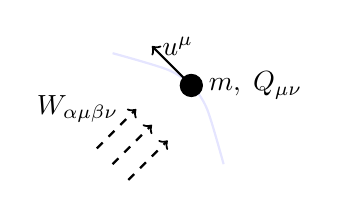
\begin{tikzpicture}
    \draw [blue!10, thick] plot [smooth] coordinates {(1.41,0) (1.2,0.7) (1,1) (0.7,1.2) (0,1.41)}; 
    \filldraw[black] ( 1, 1) circle (4pt) node[right] {$\;m,\;Q_{\mu\nu}$};
    \draw[thick, ->] ( 1, 1) -- ( 0.5, 1.5) node[right] {$u^{\mu}$};
    \draw[thick, dashed, ->] (    0,    0) -- ( 0.5, 0.5);
    \draw[thick, dashed, ->] ( -0.2,  0.2) -- ( 0.3, 0.7) node[left] {$W_{\alpha\mu\beta\nu}\;$};
    \draw[thick, dashed, ->] (  0.2, -0.2) -- ( 0.7, 0.3);
    \end{tikzpicture}
\end{document}

